\section{Evaluation}\label{sec:eval}

We evaluate \sysname{} using a combination of testbed experiments and numerical
experiments. Our evaluation focuses on three key questions: $(i)$ Can \sysname{}
prevent deadlock? $(ii)$ Is \sysname{} scalable for large data center networks?,
and $(iii)$ Is there a performance penalty with \sysname{}?

In this section, we answer these questions using a mix of tetsbed experiments
and numerical analysis.

\begin{figure}
	\centering
	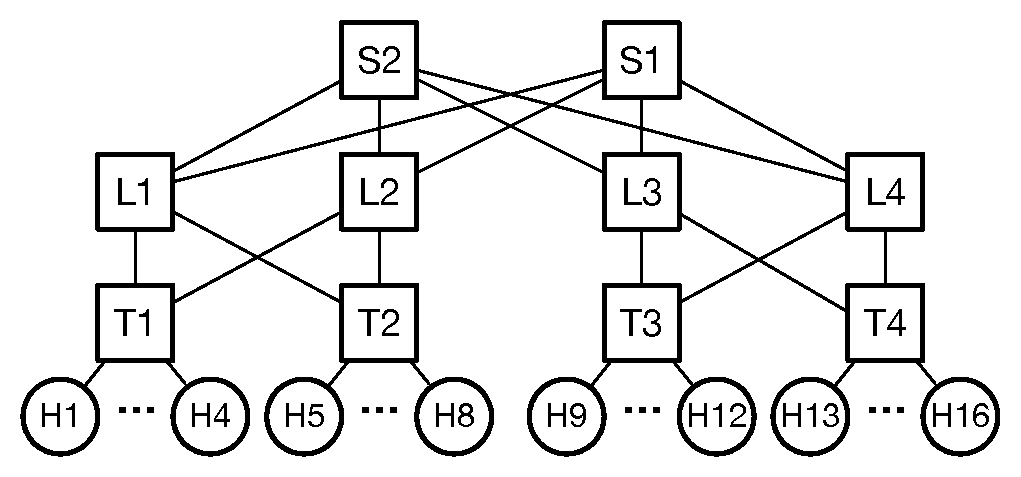
\includegraphics[width=0.45\textwidth] {figs/testbed_topo}
	\caption{Testbed Topology.}\label{fig:testbed_topo}
\end{figure}

\textbf{Testbed setup}: We use a small Clos network as our testbed with 16
servers and 10 switches, as shown in Figure~\ref{fig:testbed_topo}. Each server
is a Dell PowerEdge R730 server with a 40Gbps Mellanox ConnectX-3 Pro NIC, two
16-core Intel E5-2698 2.3GHz CPUs, 256GB memory and 2TB hard disk. Each switch
is a Arista 7060CX-32S switch with 32 100Gbps ports and 16MB packet buffer. Our
switches support PFC with at most 8 priority classes. Our ConnectX-3 Pro NICs
support RoCEv2 and DCQCN protocol.

\subsection{Deadlock prevention}\label{subsec:exp_validation}

\begin{figure}[t]
	%\vspace{-0.1in}
	\centering
	
	\subfloat[short for lof][] {
		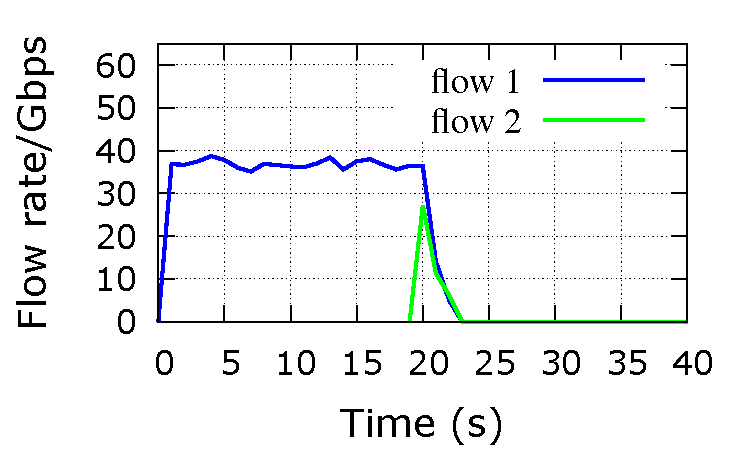
\includegraphics[width=0.25\textwidth] {figs/validation_nonloopcase_flowrate_notagger}
	}
	\subfloat[short for lof][]{
		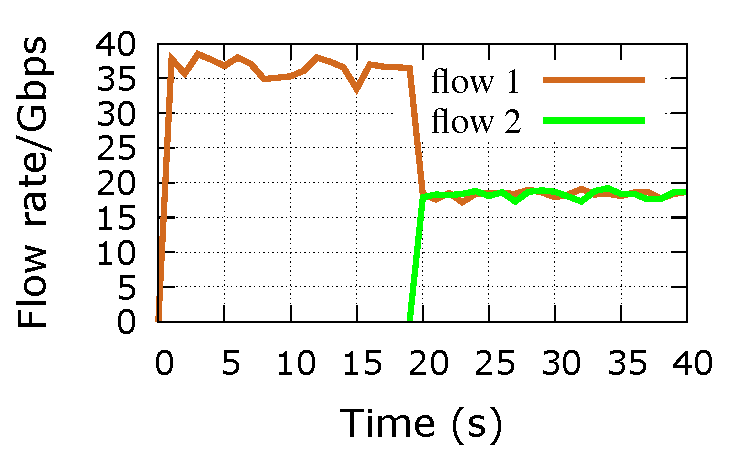
\includegraphics[width=0.25\textwidth] {figs/validation_nonloopcase_flowrate_tagger}
	}
	
	\caption{Clos deadlock due to 1 bounce paths}\label{fig:exp_validation_nonloop}
	
\end{figure}

\begin{figure}[t]
	%\vspace{-0.1in}
	\centering
	
	\subfloat[short for lof][] {
		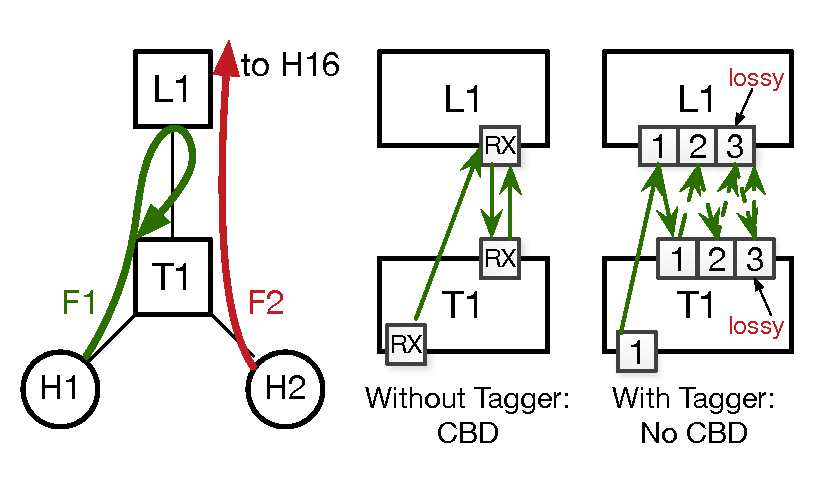
\includegraphics[width=0.2\textwidth] {figs/validation_loopcase_scenario}
	}
	\subfloat[short for lof][]{
		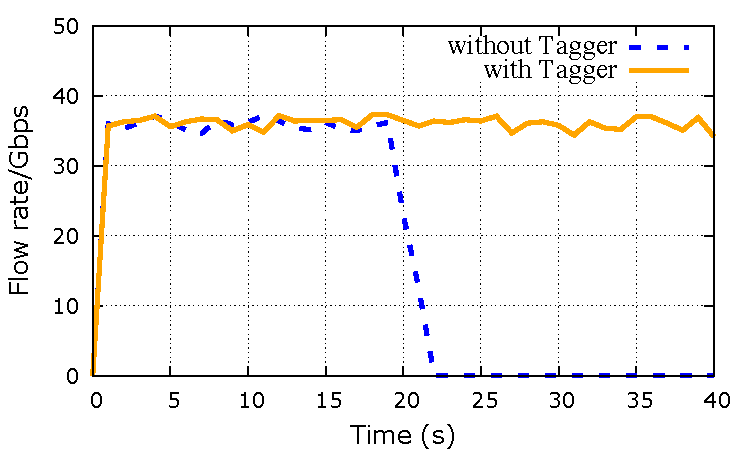
\includegraphics[width=0.3\textwidth] {figs/validation_loopcase_flowrate}
	}
	
	\caption{Deadlock due to routing loop}\label{fig:exp_validation_loop}
	
\end{figure}

We have already {\em proved} that \sysname{} prevents deadlock, so the
experiments in this section are primarily illustrative. 

\textbf{Deadlock due to one bounce:} We recreate the scenario shown in
Figure~\ref{fig:clos_1_bounce}, where 1-bounce paths lead to CBD.  In this
experiment, we start the green flow at time 0, and the blue flow at time 20.
Figure~\ref{fig:exp_validation_nonloop} shows the rate of the two flows with and
without \sysname{}.  Without \sysname{}, deadlock occurs and rate of both flows
are reduced to 0. With \sysname{}, there is no deadlock and flow rates are not
affected.

\textbf{Deadlock due to routing loop:} As shown in
Figure~\ref{fig:exp_validation_loop}(a), we generate 2 flows across different
ToRs, i.e., flow 1 from H1 to H15 and flow 2 from H2 to H16. At time = 20s, we
install a bad route at L1 to let flow 1 enter a routing loop between T1 and L1.
The path taken by flow 2 also traverses link T1-L1. 

In Figure~\ref{fig:exp_validation_loop}(b), we plot the rate of flow 2 with and
without \sysname{}. As we can see, if \sysname{} is not used, deadlock occurs
and flow 2 is paused due to propagation of PFC PAUSE. With \sysname{}, there is
no deadlock and rate of flow 2 is not affected by the routing loop.

\subsection{Scalability}
\label{subsec:exp_overhead}

As discussed in \S\ref{sec:challanges}, commodity switches can support only a
limited number of lossless queues.  We have already shown that on a Clos
topology, \sysname{} requires $k+1$ lossless priorities to support paths with
upto $k$ bounces. In this section, we consider other topologies. 

\begin{table*}[t]
	\centering
		\begin{tabular}{|r|r|r|r|r|}
			\hline
			Switch $\#$ &  Switch port $\#$ &  Network diameter &	\multicolumn{1}{c|}{\tabincell{c}{\text{$\#$ of lossless} \\ \text{priority classes}}}   &    
			\multicolumn{1}{c|}{\tabincell{c}{Max \text{$\#$ of rules at} \\
				\text{a switch}}}\\
			\hline
			\hline
			10 & 12 & 5 & 2 & 10 \\
			\hline
			100 & 32 & 6 & 3 &  37 \\
			\hline
			500 & 64 & 6 & 3 & 76 \\
			\hline
			1,000 & 64 & 6 & 3 & 88 \\
			\hline
			2,000 & 64 & 7 & 3 & 98 \\
			\hline
			
		\end{tabular}
	\caption{Resource consumption of Algorithm~\ref{alg:greedy} on Jellyfish at different scales.}
	\label{table:resource_consumption}
\end{table*}

Jellyfish topology is an r-regular random graph, characterized by the the number
of switches (N), the number of ports a switch has (k) and the number of ports
used to connect with other switches (r) (the remaining $k-r$ ports are for
servers). In our experiment, we let r = k/2.  We construct the routing paths by
building destination-rooted shortest-path spanning trees at all the servers.

Table~\ref{table:resource_consumption}, shows the number of lossless priority
classes needed for a variety of network sizes. We see that \sysname{} requires
only three classes even for a network with 2000 switches. 

The table also shows the maximum number of rules needed at a switch for various
configurations~\footnote{Different switches require different number of rules
due to the random nature of the topology.}. Even with 2000 switches, we need
just 98 ACLs at a switch. Modern commodity switches can support 1-4K
ACL~\cite{xx}, so this is not a bottleneck. 

\subsection{Performance penalty}\label{subsec:exp_performanceoverhead}

\begin{figure}
	\centering
	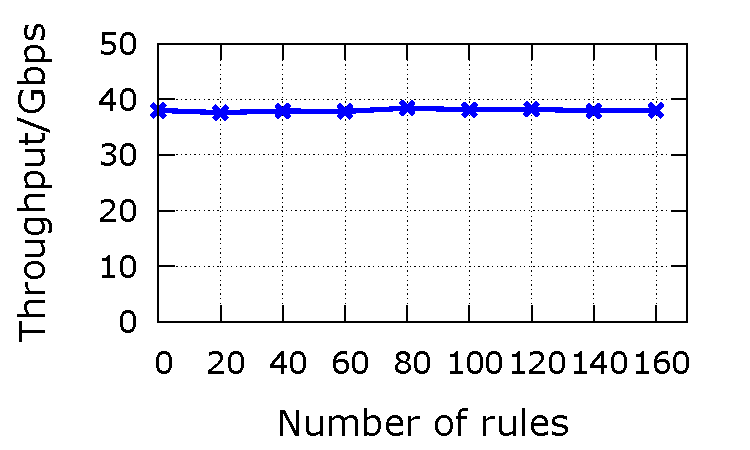
\includegraphics[width=0.45\textwidth] {figs/overhead_avgthrpt}
	\caption{Measurement of throughput overhead.}\label{fig:thrpt_overhead}
\end{figure}

\begin{table}[t]
	\centering
	\scalebox{0.9}{
	\begin{tabular}{|r|r|r|r|r|r|}
		\hline
		$\#$ of rules & Average RTT (us) &   \multicolumn{1}{c|}{\tabincell{c}{\text{50th percentile} \\ \text{RTT (us)}}}   & \multicolumn{1}{c|}{\tabincell{c}{\text{99th percentile} \\ \text{RTT (us)}}} \\
		\hline
		\hline
		10 & 77 & 81 & 104  \\
		\hline
		20 & 79 & 77 & 99  \\
		\hline
		40 & 77 & 74 & 106 \\
		\hline
		80 & 81 & 82 & 101 \\
		\hline
		160 & 75 & 77 & 104 \\
		\hline
		
	\end{tabular}
     }
	\caption{Measurement of latency overhead.}
	\label{table:latency_overhead}
\end{table}

At run time, the only performance penalty of \sysname{} is that the packet has
to traverse the ACL rules. These are installed in TCAM, and hence induce
negligible penalty, as illustrated by the following experiments.

\textbf{Throughput penalty}: We generate one flow from H1 to H2, and observe
its average throughput over 100 seconds under varying number of \sysname{} rules
installed on T1. Figure~\ref{fig:thrpt_overhead} shows that the average
throughput is not affected.

\textbf{Latency penalty}: We install different number of \sysname{} rules in T1
and collect 5000 RTT samples between H1 and H2.
Table~\ref{table:latency_overhead} shows that the number of installed rules does
not have significant impact on network latency.
